% Hlavicka pro protokoly z fyzikalniho praktika.
% Verze pro: LaTeX
% Verze hlavicky: 22. 2. 2007
% Autor: Ustav fyziky kondenzovanych latek
% Ke stazeni: www.physics.muni.cz/ufkl/Vyuka/
% Licence: volne k pouziti, nejlepe k vcasnemu odevzdani protokolu z Vaseho mereni.


\documentclass[czech,11pt,a4paper]{article}
\usepackage[T1]{fontenc}
\usepackage{graphicx, animate}
\usepackage{mathtools}
\usepackage{amssymb}
\usepackage{amsthm}
\usepackage{thmtools}
\usepackage{xcolor}
\usepackage{nameref}
\usepackage{babel}
\usepackage{hyperref}
\usepackage{multicol}
\usepackage[export]{adjustbox}
\usepackage{subcaption}
\usepackage{caption}
\usepackage{multirow}
\usepackage{float}
\usepackage{placeins}

\graphicspath{ {./images/} }
\usepackage[backend=biber,style=numeric]{biblatex}       % [1], [2], ...




\addbibresource{ref.bib}


%%% Nemente:
\usepackage[margin=2cm]{geometry}
\newtoks\jmenopraktika \newtoks\jmeno \newtoks\datum
\newtoks\obor \newtoks\skupina \newtoks\rocnik \newtoks\semestr
\newtoks\cisloulohy \newtoks\jmenoulohy

%%% Nemente - konec.


%%%%%%%%%%% Doplnte pozadovane polozky:

\jmenopraktika={Fyzikální praktikum 3}  % nahradte jmenem vaseho predmetu
\jmeno={Teodor Duraković}            % nahradte jmenem mericiho
\datum={27.~března 2024}        % nahradte datem mereni ulohy
\obor={F}                     % nahradte zkratkou vami studovaneho oboru
\skupina={Út 14:00}            % nahradte dobou vyuky vasi seminarni skupiny
\rocnik={II}                  % nahradte rocnikem, ve kterem studujete
\semestr={IV}                 % nahradte semestrem, ve kterem studujete

\cisloulohy={7}               % nahradte cislem merene ulohy
\jmenoulohy={Určení teploty elektrického oblouku}           % nahradte vlhkosti vzduchu pri mereni (v %)

%%%%%%%%%%% Konec pozadovanych polozek.


%%%%%%%%%%% Uzitecne balicky:

%%%%%% Zamezeni parchantu:
\widowpenalty 10000 \clubpenalty 10000 \displaywidowpenalty 10000
%%%%%% Parametry pro moznost vsazeni vetsiho poctu obrazku na stranku
\setcounter{topnumber}{3}	  % max. pocet floatu nahore (specifikace t)
\setcounter{bottomnumber}{3}	  % max. pocet floatu dole (specifikace b)
\setcounter{totalnumber}{6}	  % max. pocet floatu na strance celkem
\renewcommand\topfraction{0.9}	  % max podil stranky pro floaty nahore
\renewcommand\bottomfraction{0.9} % max podil stranky pro floaty dole
\renewcommand\textfraction{0.1}	  % min podil stranky, ktery musi obsahovat text
\intextsep=8mm \textfloatsep=8mm  %\intextsep pro ulozeni [h] floatu a \textfloatsep pro [b] or [t]

% Tecky za cisly sekci:
\renewcommand{\thesection}{\arabic{section}.}
\renewcommand{\thesubsection}{\thesection\arabic{subsection}.}
\renewcommand{\thesubsubsection}{\thesubsection\arabic{subsubsection}.}
% Jednopismenna mezera mezi cislem a nazvem kapitoly:
\makeatletter \def\@seccntformat#1{\csname the#1\endcsname\hspace{1ex}} \makeatother


%%%%%%%%%%%%%%%%%%%%%%%%%%%%%%%%%%%%%%%%%%%%%%%%%%%%%%%%%%%%%%%%%%%%%%%%%%%%%%%
%%%%%%%%%%%%%%%%%%%%%%%%%%%%%%%%%%%%%%%%%%%%%%%%%%%%%%%%%%%%%%%%%%%%%%%%%%%%%%%
% Zacatek dokumentu
%%%%%%%%%%%%%%%%%%%%%%%%%%%%%%%%%%%%%%%%%%%%%%%%%%%%%%%%%%%%%%%%%%%%%%%%%%%%%%%
%%%%%%%%%%%%%%%%%%%%%%%%%%%%%%%%%%%%%%%%%%%%%%%%%%%%%%%%%%%%%%%%%%%%%%%%%%%%%%%

\begin{document}
	
	%%%%%%%%%%%%%%%%%%%%%%%%%%%%%%%%%%%%%%%%%%%%%%%%%%%%%%%%%%%%%%%%%%%%%%%%%%%%%%%
	% Nemente:
	%%%%%%%%%%%%%%%%%%%%%%%%%%%%%%%%%%%%%%%%%%%%%%%%%%%%%%%%%%%%%%%%%%%%%%%%%%%%%%%
	\thispagestyle{empty}
	
	{
		\begin{center}
			\sf 
			{\Large Ústav fyziky a technologií plazmatu Přírodovědecké fakulty Masarykovy univerzity} \\
			\bigskip
			{\huge \bfseries FYZIKÁLNÍ PRAKTIKUM} \\
			\bigskip
			{\Large \the\jmenopraktika}
		\end{center}
		
		\bigskip
		
		\sf
		\noindent
		\setlength{\arrayrulewidth}{1pt}
		\begin{tabular*}{\textwidth}{@{\extracolsep{\fill}} l l}
			\large {\bfseries Zpracoval:}  \the\jmeno & \large  {\bfseries Naměřeno:} \the\datum\\[2mm]
			\large  {\bfseries Obor:} \the\obor  \hspace{40mm}  {\bfseries Skupina:} \the\skupina %
			%{\bfseries Ročník:} \the\rocnik \hspace{5mm} {\bfseries Semestr:} \the\semestr  
			&\large {\bfseries Testováno:}\\
			\\
			\hline
		\end{tabular*}
	}
	
	\bigskip
	
	{
		\sf
		\noindent \begin{tabular}{p{3cm} p{0.6\textwidth}}
			\Large  Úloha č. {\bfseries \the\cisloulohy:} \par
			\smallskip
			&\Large \bfseries \the\jmenoulohy  \\[2mm]
		\end{tabular}
	}
	
	\vskip1cm
	
	%%%%%%%%%%%%%%%%%%%%%%%%%%%%%%%%%%%%%%%%%%%%%%%%%%%%%%%%%%%%%%%%%%%%%%%%%%%%%%%
	% konec Nemente.
	%%%%%%%%%%%%%%%%%%%%%%%%%%%%%%%%%%%%%%%%%%%%%%%%%%%%%%%%%%%%%%%%%%%%%%%%%%%%%%%
	
	%%%%%%%%%%%%%%%%%%%%%%%%%%%%%%%%%%%%%%%%%%%%%%%%%%%%%%%%%%%%%%%%%%%%%%%%%%%%%%%
	%%%%%%%%%%%%%%%%%%%%%%%%%%%%%%%%%%%%%%%%%%%%%%%%%%%%%%%%%%%%%%%%%%%%%%%%%%%%%%%
	% Zacatek textu vlastniho protokolu
	%%%%%%%%%%%%%%%%%%%%%%%%%%%%%%%%%%%%%%%%%%%%%%%%%%%%%%%%%%%%%%%%%%%%%%%%%%%%%%%
	%%%%%%%%%%%%%%%%%%%%%%%%%%%%%%%%%%%%%%%%%%%%%%%%%%%%%%%%%%%%%%%%%%%%%%%%%%%%%%%
	
	\begin{multicols}{2}
		\section{Zadání}
		1. Identifikujte spektrální čáry emitované parami materiálu elektrod v obloukovém výboji a určete jejich intenzitu. Ze sklonu pyrometrické přímky určete teplotu oblouku. \\
		2. Určete z naměřeného molekulového spektra radikálu OH rotační teplotu.
		
		
		\section{Teorie}
		
		
		
		Látky excitované na vyšší energetické hladiny mohou svoji energii předat okolí ve formě záření. Pokud se elektron v atomech nebo molekulách přechodem na nižší hladinu deexituje, je vyzářen foton s energií odpovídající rozdílu hladin:
		
		
		\begin{equation}
			h \nu = E_m - E_n = \frac{hc}{\lambda_{mn}}
		\end{equation}
		
		
		Tuto vlastnost využívá optická emisní spektroskopie (OES), která analyzuje záření vzniklé ve vysoce energetických prostředích jako je plazma. Podle struktury spektra lze odlišit typy zářící látky: u atomů vzniká čárové spektrum, u molekul pásové, u pevných látek spojité.
		
		Tato úloha se skládá ze dvou částí. V první určujeme \textbf{excitační teplotu par železa} v obloukovém výboji. Ve druhé vyhodnocujeme \textbf{rotační teplotu radikálu OH} v neizotermickém plazmatu.
		
		\subsection{Excitační teplota atomů železa}
		
		Pro relativní intenzitu spektrální čáry platí vztah:
		
		\begin{equation}			
			I_{mn} \sim \frac{A_{mn} g_m}{\lambda_{mn}} \cdot \exp\left(-\frac{E_m}{kT}\right)		
		\end{equation}
		
		kde $I_{mn}$ je relativní intenzita čáry, $\lambda_{mn}$ vlnová délka, $A_{mn}$ pravděpodobnost přechodu (Einsteinův koeficient), $g_m$ statistická váha horní hladiny, $E_m$ excitační energie horní hladiny a $k$ je Boltzmannova konstanta, $T$ teplota.
		
		
		Po úpravách získáme vztah vhodný pro lineární závislost tzv. pyrometrické přímky:
		
		
		\begin{equation}
			\ln\left(\frac{I_{mn} \cdot \lambda_{mn}}{A_{mn} g_m}\right) = -\frac{E_m}{kT} + \text{konst}
		\end{equation}
		
		
		Z naměřených relativních intenzit, známých vlnových délek, energií a přechodových pravděpodobností lze tak sestavit lineární závislost a určit teplotu z její směrnice.
		
		\subsection{Rotační teplota molekuly OH}
		
		Dvouatomová molekula má oproti atomům navíc vibrační a rotační stupně volnosti. Celková energie jejího stavu je dána jako součet:
		
		
		\begin{equation}
			E = E_e + E_v(\nu) + E_r(N)
		\end{equation}
		
		
		kde $E_e$ je energie elektronového stavu, $E_v(\nu)$ vibrační energie (v aproximaci anharmonického oscilátoru) a $E_r(N)$ rotační energie (v aproximaci netuhého rotátoru). Pro rotační energii platí:
		
		
		\begin{equation}
			E_r(N) = hc \cdot \left[B_\nu N(N+1) - D_e N^2(N+1)^2\right]
		\end{equation}
		
		
		Základ pro výpočet rotační teploty tvoří intenzity rotačních čar:
		
		
		\begin{equation}
			I_{J'} \propto \tilde{\nu}^4 S_{J'J''} \cdot \exp\left(-\frac{B' hc N'(N'+1)}{kT}\right)
		\end{equation}
		
		
		Po logaritmování opět dostáváme lineární vztah, jehož směrnice umožňuje výpočet teploty:
		
		
		\begin{equation}
			\ln\left(\frac{I_{J'}}{\tilde{\nu}^4 S_{J'J''}}\right) = -\frac{B' hc}{kT} N'(N'+1) + \text{konst}
		\end{equation}
		
		
		kde $\tilde{\nu}$ je vlnočet čáry, $S_{J'J''}$ je Hoenl-Londonův faktor, $B'$ rotační konstanta horního vibračního stavu a $N'$ je rotační kvantové číslo (v této úloze platí $N' = J' - 1/2$).
		
		
		\subsection{Vyhodnocení a software}
		
		Při praktickém vyhodnocení se provádí je nutná správná identifikace spektrálních čar (včetně případného posunu) a odečtení temného proudu. Zatímco Temný proud lze eliminovat bez referenčních dat, posun spektrálních čar je nutno vyvodit za pomocí reference.

		
		Pro identifikaci rotační struktury spektra OH se využívá programů \textbf{SPAN 1.7} a \textbf{Lifbase 2.1} – první umožňuje analýzu naměřeného spektra, druhý poskytuje simulované spektrum pro orientaci. Hodnota rotační konstanty použitá v úloze je:
		
		\[
		B' = 1696.6\ \text{cm}^{-1}
		\]
		
		
		\section{Zpracování dat}
		\subsection{Excitační teplota atomů železa}
		Zpracováváme soubor \verb*|data3|, pracujeme se spektrem viditelným na obr. 1.
		\begin{figure}[H]
			\centering
			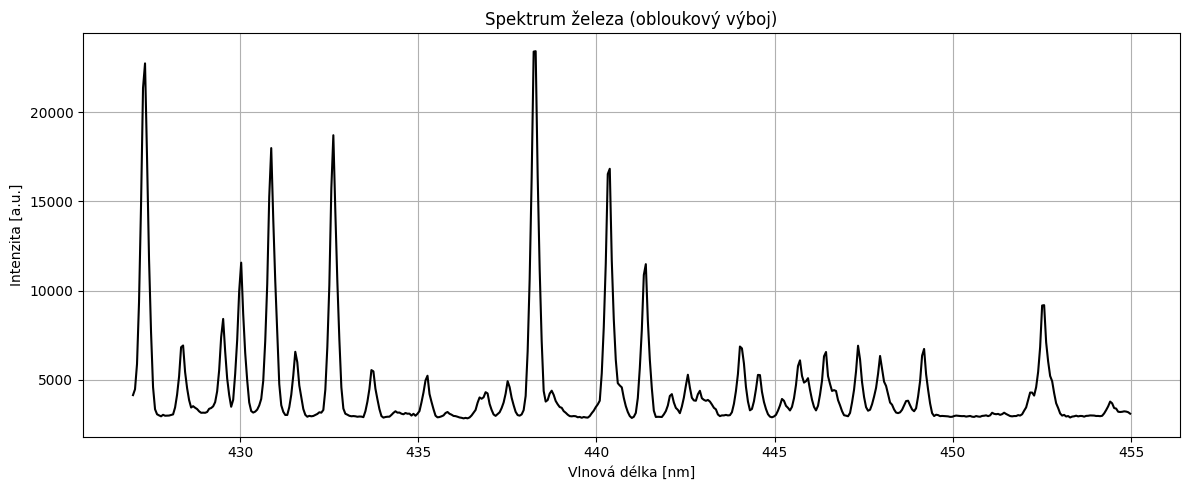
\includegraphics[width=0.9\linewidth]{spectrum}
			\caption{Spektrum obloukového výboje železa - závislost rel. intenzity na vlnové délce}

		\end{figure}
		Pro kompenzaci temného proudu využíváme oblasti bez spektrálních čar. Detekcí vrcholů nalezneme potenciální spektrální čáry, poté je přiřadíme k tabulce v návodu\cite{navod}. Získáváme data na obr. 2:
		
		\begin{figure}[H]
			\centering
			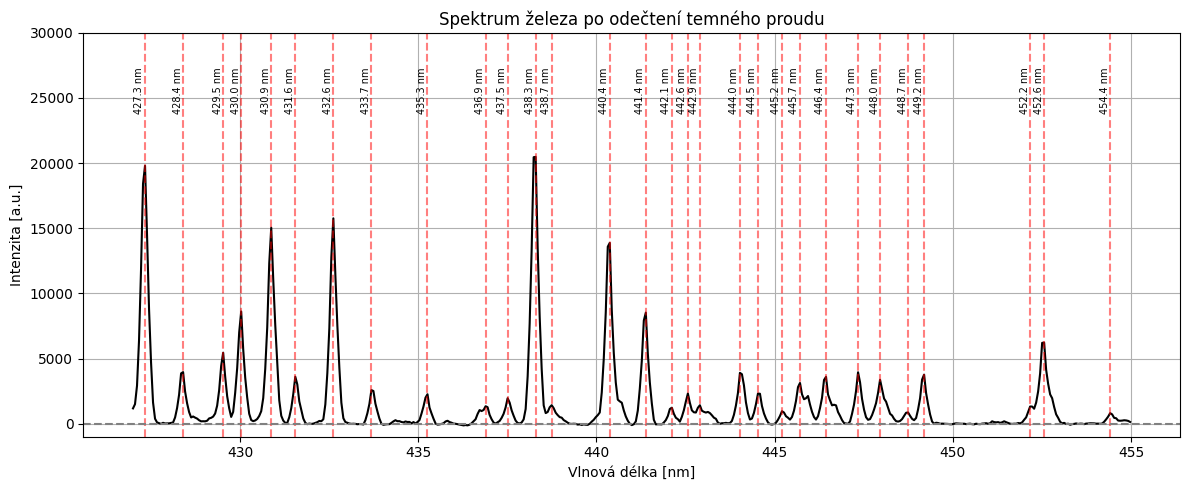
\includegraphics[width=0.9\linewidth]{spectrum2}
			\caption{Spektrum obloukového výboje železa - po odstranění temného proudu a detekci špiček}

		\end{figure}
		
		Následně přiřazujeme detekované čáry k referenčním čarám v návodu, pro získání rel. intenzity integrujeme oblast pod špičkou. Pro integraci je nutno vymezit meze samotné čáry - jelikož se proces snažíme algoritmizovat a data nezpracovávat manuálně, meze definujeme tak, že pro každou čáru detekujeme i Full Width Half Maxmum a samotné meze jako body vzdálené od středu o $1.625\cdot \mathrm{FWHM}$. Zpracováním získáváme výsledek viditelný na obr. 3.
		\begin{figure}[H]
			\centering
			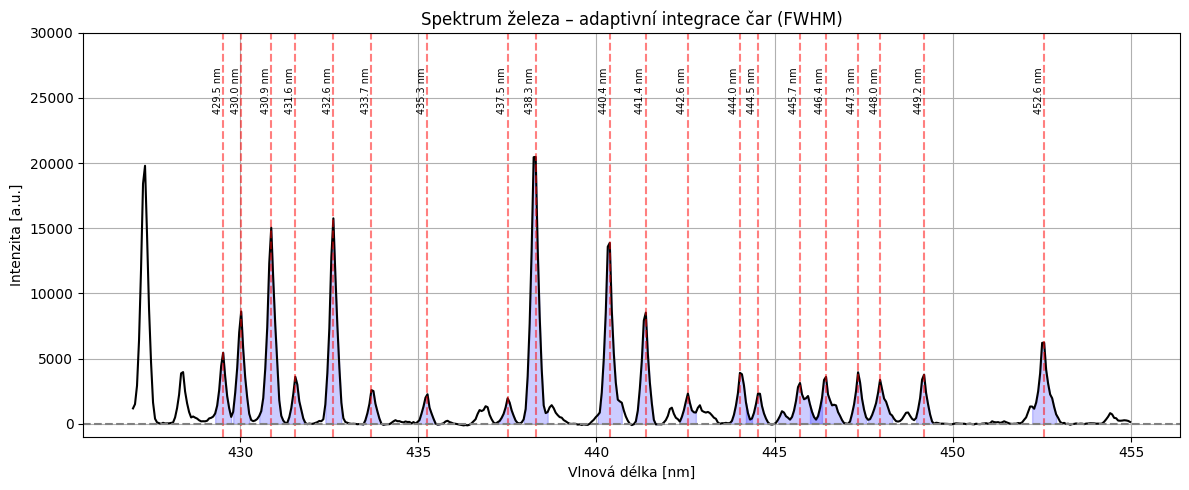
\includegraphics[width=0.9\linewidth]{spectrum3}
			\caption{Spektrum obloukového výboje železa - fialové oblasti znázorňují meze integrace}			
		\end{figure}
		Zároveň lze měřit odchylku detekovaných čar od čar referenčních, získáváme $\Delta \lambda = 0.084\pm 0.151$. Odchylka od referenčních dat tedy není primárně způsobena posunem celého spektra. Ze závislosti odchylky na vlnové délce pozorujeme, že s rostoucí vlnovou délkou roste i odchylka (obr. 4). Lze tedy předpokládat, že jsou data "roztažena", odchylka roste od bodu, který jsme lineární regresí získali jako průsečík osy x.
		\begin{figure}[H]
			\centering
			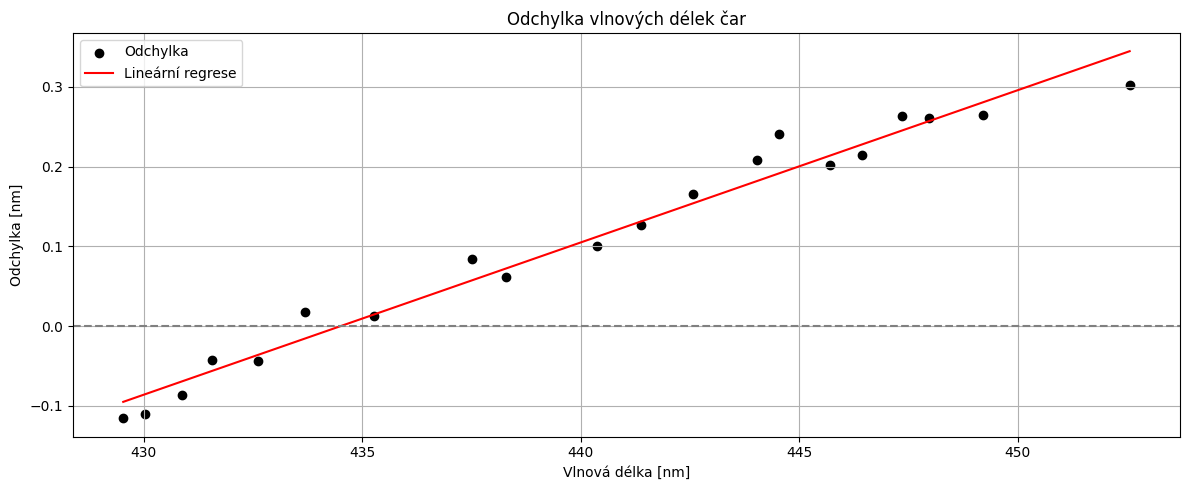
\includegraphics[width=0.9\linewidth]{zavislost}
			\caption{Závislost odchylky měřené vlnové délky od délky referenční}			
		\end{figure}
		Se získanými relativními intenzitami je nicméně možno určit teplotu výboje. Použitím formule (3), resp. vykreslením pyrometrické přímky (obr. 5), odhadujeme teplotu.
		\begin{figure}[H]
			\centering
			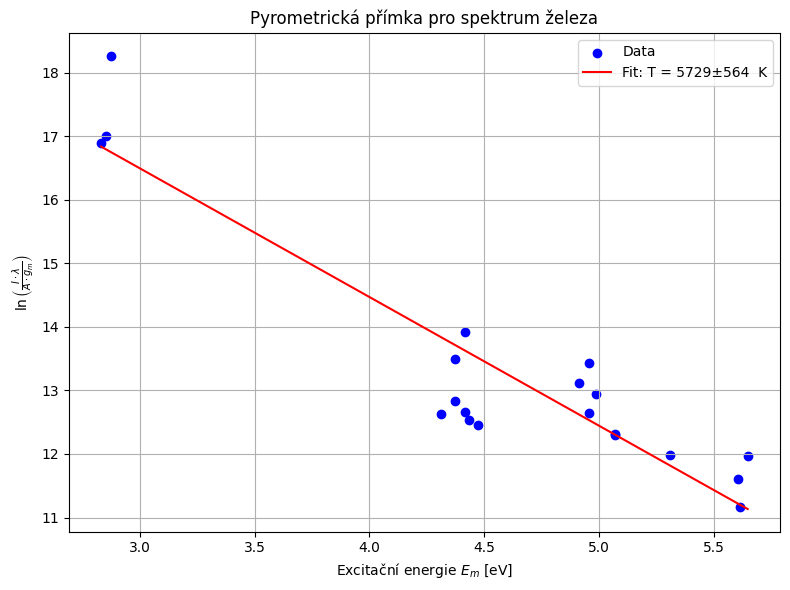
\includegraphics[width=0.9\linewidth]{pyrometrika}
			\caption{Pyrometrická přímka obloukového výboje železa}			
		\end{figure}
		\begin{equation*}
			T_{\mathrm{Fe}} = 5729 \pm 564 \,\mathrm{K}
		\end{equation*}
		\subsection{Rotační teplota molekuly OH}
		Pro analýzu spektra molekuly OH nejdříve generujeme referenční data tak, jak je uvedeno v návodu. Okamžitě pozorujeme velký rozdíl mezi měřenými a referenčními (simulovanými) daty, jak je vidět na Obr. 6, odchylka zde dosahuje až několika nanometrů.
		\begin{figure}[H]
			\centering
			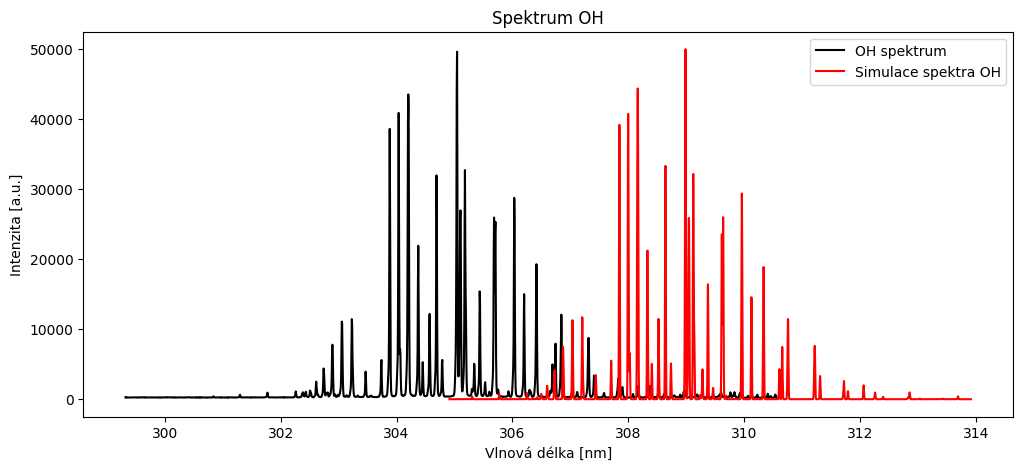
\includegraphics[width=0.9\linewidth]{srovnani}
			\caption{Naměřené a simulované spektrum OH}			
		\end{figure}
		Kalibraci provádíme obdobným způsobem, jako v předchozí úloze. Srovnáním největších špiček určíme odchylku, lineárním fitem závislosti odchylky na vlnové délce (původní, nekalibrované) z konstant regrese určíme kalibrační funkci, kterou aplikujeme na původní vlnové délky naměřených dat. Zároveň odstraňujeme hodnoty temného proudu, stejným způsobem jako v předchozí úloze. Srovnání kalibrovaného a simulovaného spektra je tímto úspěšně provedeno, jak lze ověřit na Obr. 7.
		\begin{figure}[H]
			\centering
			\includegraphics[width=0.9\linewidth]{Spectrum4}
			\caption{Kalibrované a simulované spektrum OH}			
		\end{figure}
		Nyní referenční data z tabulky návodu přiřadíme konkrétním čarám, integrací získáme jejich rel. intenzitu a znovu můžeme určit rotační teplotu pyrometrickou přímkou (obr. 8)
		\begin{figure}[H]
			\centering
			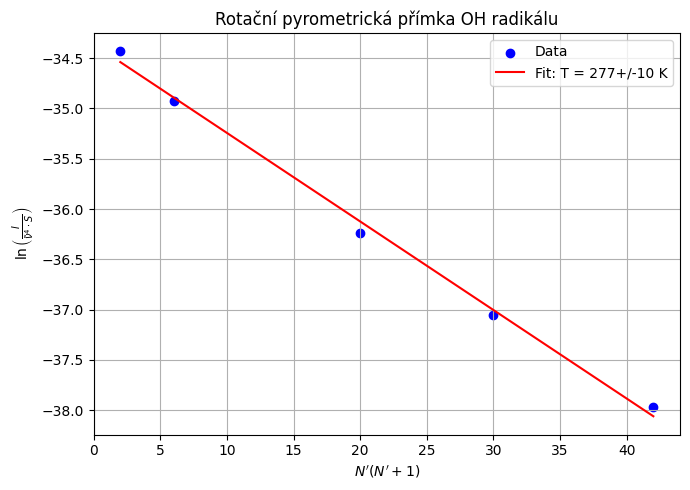
\includegraphics[width=0.9\linewidth]{pyrometrika2}
			\caption{Pyrometrická přímka OH radikálu}			
		\end{figure}
		\begin{equation*}
			T_{\mathrm{OH} = 280 \pm 1 \,\mathrm{K}}
		\end{equation*}
		\subsubsection{Zpracování dat v programu SPAN}
		
		Pro výpočet rotační teploty molekuly OH data znovu importujeme, v programu dle instrukcí označíme pouze radikál OH, následně identifikujeme konkrétní čáry. Následně lze automaticky ze spektra kalibrovat graf, teplota je vypočtena automaticky. Získáváme:
		\begin{equation*}
			T_{\mathrm{OH}}= 300 \pm 16 \,\mathrm{K}
		\end{equation*}
		
		
		
		
		\section{Závěr}
		Úspěšně se nám podařilo stanovit teplotu elektrického výboje Fe - získaná hodnota pro teplotu výboje dává smysl. Stejně tak se nám podařilo určit rotační teplotu molekuly OH, jejíž hodnotu se nám zároveň podařilo ověřit, respektive replikovat, softwarem SPAN.
		
\printbibliography
\newpage

			\end{multicols}
			\section{Příloha}
			\begin{table}[H]
				\centering
				\caption{Naměřené a referenční hodnoty spektrálních čar železa včetně intenzit a dalších parametrů.}
				\label{tab:zelezo_spektrum}
				\begin{tabular}{lrlllrl}
					$\lambda_\mathrm{naměř.}$ [nm] &  $I_\mathrm{max}$ [a.u.] &  $\lambda_\mathrm{ref}$ [nm] &  $E_m$ [eV] &  $A_m g_m$ [$10^8\,\mathrm{s}^{-1}$] &  $I_\mathrm{int}$ [a.u.] &  $\Delta \lambda$ [nm] \\  \hline                    429.5289 &              5451.388889 &                      429.413 &       4.371 &                               0.7100 &              1203.107744 &                -0.1159 \\                      430.0347 &              8610.388889 &                      429.924 &       5.308 &                               5.2000 &              1931.572144 &                -0.1107 \\                 430.8777 &             15041.388889 &                      430.791 &       4.434 &                               5.9000 &              3821.806067 &                -0.0867 \\                       431.5521 &              3606.388889 &                      431.509 &       5.070 &                               1.5000 &               765.422144 &                -0.0431 \\                       432.6198 &             15763.388889 &                      432.576 &       4.473 &                               6.1000 &              3630.195206 &                -0.0438 \\                       433.6876 &              2578.388889 &                      433.705 &       4.415 &                               0.2300 &               584.124067 &                 0.0174 \\                       435.2611 &              2262.388889 &                      435.274 &       5.070 &                               1.0000 &               511.688678 &                 0.0129 \\                       437.5088 &              1956.388889 &                      437.593 &       2.832 &                               0.0094 &               466.247128 &                 0.0842 \\                       438.2954 &             20480.388889 &                      438.357 &       4.312 &                               7.7000 &              5367.759939 &                 0.0616 \\                       440.3742 &             13880.388889 &                      440.475 &       4.371 &                               4.4000 &              3722.427900 &                 0.1008 \\                       441.3855 &              8525.388889 &                      441.512 &       4.415 &                               2.8000 &              1992.000750 &                 0.1265 \\                        442.5652 &              2317.388889 &                      442.731 &       2.851 &                               0.0099 &               538.930667 &                 0.1658 \\                        444.0256 &              3902.388889 &                      444.234 &       4.988 &                               1.1000 &              1030.196411 &                 0.2084 \\                        444.5311 &              2309.388889 &                      444.772 &       5.009 &                               1.1000 &               669.295872 &                 0.2409 \\                        445.7104 &              3126.388889 &                      445.912 &       4.955 &                               1.0000 &              1532.649372 &                 0.2016 \\                        446.4405 &              3595.388889 &                      446.655 &       5.606 &                               5.3000 &              1298.992717 &                 0.2145 \\                        447.3389 &              3947.388889 &                      447.602 &       5.614 &                               5.4000 &               852.832389 &                 0.2631 \\                        447.9565 &              3371.388889 &                      448.217 &       2.875 &                               0.0053 &              1016.836294 &                 0.2605 \\                      449.1917 &              3767.388889 &                      449.457 &       4.955 &                               1.2200 &               844.602400 &                 0.2653 \\                        452.5592 &              6224.388889 &                      452.862 &       4.913 &                               1.8000 &              1978.389039 &                 0.3028 \\
				\end{tabular}
			\end{table}
			
			\begin{table}[H]
				\centering
				\caption{Naměřené spektrální čáry radikálu OH a hodnoty potřebné pro určení rotační teploty.}
				\label{tab:oh_spektrum}
				\begin{tabular}{lrllllll}

					$\lambda_\mathrm{naměř.}$ [nm] &
					$I_\mathrm{max}$ [a.u.] &
					$\lambda_\mathrm{ref}$ [nm] &
					$N'$ &
					$S_{J'J''}$ &
					$I_\mathrm{int}$ [a.u.] &
					$N'(N'+1)$ &
					$\ln \left(\frac{I_\mathrm{int}}{\tilde\nu^4 S_{J'J''}}\right)$ \\
					\hline

					307.846 & 38365.416 & 307.843 & 1.0 & 0.563 & 699.391 & 2.0 & -34.429 \\
					307.997 & 40643.416 & 307.996 & 2.0 & 1.065 & 803.388 & 6.0 & -34.926 \\
					308.329 & 21662.749 & 308.326 & 4.0 & 2.100 & 425.078 & 20.0 & -36.237 \\
					308.521 & 11930.749 & 308.512 & 5.0 & 2.640 & 235.717 & 30.0 & -37.053 \\
					308.736 &  5361.082 & 308.733 & 6.0 & 3.160 & 112.294 & 42.0 & -37.972 \\

				\end{tabular}
			\end{table}
			
		
		
		% Nakonec nezapomeňte projet text programem vlna nebo vlnka, např.
		% 	vlna -m -l -n mojeuloha.tex
		% nebo zkontrolovat a opravit jednopísmenné předložky na koncích řádků ručně.

\end{document}
